\documentclass[11pt, a4paper]{MATH2023}
\usepackage{fancyhdr}
\usepackage{setspace}
\usepackage{amsmath,mathrsfs}
\usepackage{multicol}
\usepackage{amssymb}
\usepackage{graphicx}
\usepackage{caption}
\usepackage{subcaption}
\usepackage{xcolor}
\usepackage{enumitem}
\usepackage{tikz}
\usepackage{mathtools}
\usetikzlibrary{matrix}
\usepackage[normalem]{ulem}
\usepackage{multirow}
\usepackage[linesnumbered, ruled, boxed]{algorithm2e}
\SetKwRepeat{Do}{do}{while}
\newcommand{\eg}{\textbf{[Example.] }}
\newcommand{\sol}{\textbf{[Solution.] }}
\newcommand{\ii}{{\bf i}}
\newcommand{\jj}{{\bf j}}
\newcommand{\kk}{{\bf k}}
\newcommand{\rr}{{\bf r}}
\newcommand{\FF}{{\bf F}}
\renewcommand{\div}{{\rm div\ }}
\newcommand{\curl}{{\rm curl\ }}
\newcommand{\pt}{\partial}


\title{Chapter 15}
\subtitle{Vector Field}

\begin{document}
\begin{spacing}{1.3}

    \section{Intro. to Vector Field}

    So far, we have learned two kinds of functions involving vector: 
    \begin{itemize}
        \item ${\bf r}(t)=x(t){\bf i}+y(t){\bf j}+z(t){\bf k}$: for each $t$, provides a {\it position} vector 
        $<x(t), y(t), z(t)>$, so this is a (parametric) curve.
        \item $z=f({\bf r})=f(x_1,x_2,\cdots,x_n)$: for a given vector ${\rm r}$, this gives a real number,
        so this is a function of {\it several variables}. This is also a {\bf scalar field} since for 
        any point ${\bf r}$ in {\bf field}, it gives a scalar value. 
    \end{itemize}
    Now we are looking at {\bf vector-valued} function ${\bf F}$ of a vector ${\bf r}$, i.e., ${\bf F(r)}$.
    This is a {\bf vector field}, which means for any point ${\bf r}$ in {\bf field}, it gives a vector 
    ${\bf F(r)}$. 

    You can consider a world map showing the {\it speed} and {\it direction} of wind.
    \begin{center}
        \includegraphics[scale=0.17]{images/Ch15-wind.JPG}
    \end{center}

    You can see that in a 2D map(like above), if we put a vector on each point, the vector must have 
    same dimension as the map, i.e., all vectors must also be 2D vectors.
    $${\bf F(r)}=\left\{
        \begin{array}{lll}
            (F_1({\bf r}), F_2({\bf r})) & {\bf r}=(x,y) & {\blue 2D}\\
            (F_1({\bf r}), F_2({\bf r}), F_3({\bf r})) & {\bf r}=(x,y,z) & {\blue 3D}\\
            (F_1({\bf r}), F_2({\bf r}), \cdots, F_n({\bf r})) & {\bf r}=(x_1, x_2,\cdots, x_n) & {\blue nD}
        \end{array}\right.$$
    {\bf Summary:} {\it dimension of ${\bf F}$ must be the same as ${\bf r}$.}

    \vspace{0.5in}
    {\blue This is an example of vector field.}

    \eg Assume a vector field: ${\bf F}(x,y)=\dfrac{y\ii -x\jj}{\sqrt{x^2+y^2}}$.

    \sol Notice that $||{\bf F}||=\dfrac{y^2}{x^2+y^2}+\dfrac{x^2}{x^2+y^2}=1$, all vectors 
    ${\bf F}(x,y)$ are unit vectors. Moreover, let ${\bf r}=(x,y)$, then ${\bf r}\cdot {\bf F}=0$,
    so ${\bf r}\bot {\bf F}$.

    So all vectors are unit vectors tangent to circles centered at the origin with radius $\sqrt{x^2+y^2}$.
    \begin{center}
        \includegraphics[scale=0.4]{images/Ch15-ex1.2.png}
    \end{center}

    \newpage
    \section{Divergence and Curl}

    Recall that the {\bf gradient operator} is a {\it vector operator}:
    $$\nabla =\left(\frac{\pt}{\pt x}, \frac{\pt}{\pt y}, \frac{\pt}{\pt z}\right)\qquad {\blue \rm (a\ vector)}$$

    If $\FF (\rr)=F_1(\rr)\ii +F_2(\rr) \jj +F_3(\rr) \kk$, then we define: 
    \begin{itemize}
        \item {\bf divergence} of $\FF$, written $\div \FF$:   
        $$\boxed{
        \operatorname{div} \mathbf{F}=\nabla \cdot \mathbf{F}=\frac{\partial F_1}{\partial x}+\frac{\partial F_2}{\partial y}+\frac{\partial F_3}{\partial z}
        }$$
        \item {\bf curl} of $\FF$, written $\curl \FF$: 
        $$\boxed{
        \operatorname{curl} \mathbf{F}=\nabla \times \mathbf{F}=\left|\begin{array}{ccc}
        \mathbf{i} & \mathbf{j} & \mathbf{k} \\
        \dfrac{\partial}{\partial x} & \dfrac{\partial}{\partial y} & \dfrac{\partial}{\partial z} \\
        F_1 & F_2 & F_3
        \end{array}\right|=\left(\frac{\partial h}{\partial y}-\frac{\partial g}{\partial z}\right) \mathbf{i}-\left(\frac{\partial h}{\partial x}-\frac{\partial f}{\partial z}\right) \mathbf{j}+\left(\frac{\partial g}{\partial x}-\frac{\partial f}{\partial y}\right) \mathbf{k}
        }$$
    \end{itemize}

    {\blue This example shows basic computation of {\bf divergence} and {\bf curl}.}

    \eg Let $\mathbf{r}=x \mathbf{i}+y \mathbf{j}+z \mathbf{k}$ and $\mathbf{u}=a \mathbf{i}+b \mathbf{j}+c \mathbf{k}$, where $a, b$ and $c$ are constants, show that

    (a) $\nabla \cdot \mathbf{r}=3$\\
    (b) $\nabla \times \mathbf{r}=\mathbf{0}$\\
    (c) $\nabla \cdot(\mathbf{u} \times \mathbf{r})=0$\\
    (d) $\nabla \times(\mathbf{u} \times \mathbf{r})=2 \mathbf{u}$.

    \sol 
    (a) $\disp \nabla \cdot \mathbf{r}=\left(\mathbf{i} \frac{\partial}{\partial x}+\mathbf{j} \frac{\partial}{\partial y}+\mathbf{k} \frac{\partial}{\partial z}\right) \cdot(x \mathbf{i}+y \mathbf{j}+z \mathbf{k})=
    \frac{\partial x}{\partial x}+\frac{\partial y}{\partial y}+\frac{\partial z}{\partial z}=3$\\
    (b) $\disp \nabla \times \mathbf{r}=\left|\begin{array}{ccc}
            \mathbf{i} & \mathbf{j} & \mathbf{k} \\ 
            \frac{\partial}{\partial x} & \frac{\partial}{\partial y} & \frac{\partial}{\partial z} \\ 
            x & y & z
        \end{array}\right|=\mathbf{0}$

    (c) $\disp \mathbf{u} \times \mathbf{r}=\left|\begin{array}{ccc}
            \mathbf{i} & \mathbf{j} & \mathbf{k} \\ 
            a & b & c \\ 
            x & y & z
        \end{array}\right|=(b z-c y) \mathbf{i}-(a z-c x) \mathbf{j}+(a y-b x) \mathbf{k}$

    $\disp \therefore \nabla \cdot(\mathbf{u} \times \mathbf{r})=\frac{\partial}{\partial x}(b z-c y)-\frac{\partial}{\partial y}(a z-c x)+\frac{\partial}{\partial z}(a y-b x)=0$

    (d) $\disp \nabla \times(\mathbf{u} \times \mathbf{r})=\left|\begin{array}{ccc}\mathbf{i} & \mathbf{j} & \mathbf{k} \\ \frac{\partial}{\partial x} & \frac{\partial}{\partial y} & \frac{\partial}{\partial z} \\ b z-c y & -a z+c x & a y-b x\end{array}\right|=2(a \mathbf{i}+b \mathbf{j}+c \mathbf{k})=2 \mathbf{u}$


    \newpage
    \subsection{Interpretation of Divergence}

    \newcommand{\uu}{{\bf u}}

    Imagine water in a bath tank, if the {\bf velocity} of water at any point 
    of the tank is given by $$\uu (\rr)=u_1(\rr) \ii +u_2(\rr) \jj + u_3(\rr)\kk$$
    then {\bf net outward flux per unit volume} is $\div \uu =\nabla \cdot \uu$.
    \begin{center}
        \includegraphics[scale=0.18]{images/Ch15-bath.JPG}
    \end{center}
    Moreover, 
    \begin{itemize}
        \item If more water comes inside, then $\div \uu <0$
        \item If more water comes outside, then $\div \uu >0$
        \item If the amount of water comes inside equals to comes outside, then $\div \uu =0$
    \end{itemize}

    \newpage
    {\blue This page proves the interpretation of divergence.}
    \begin{center}
    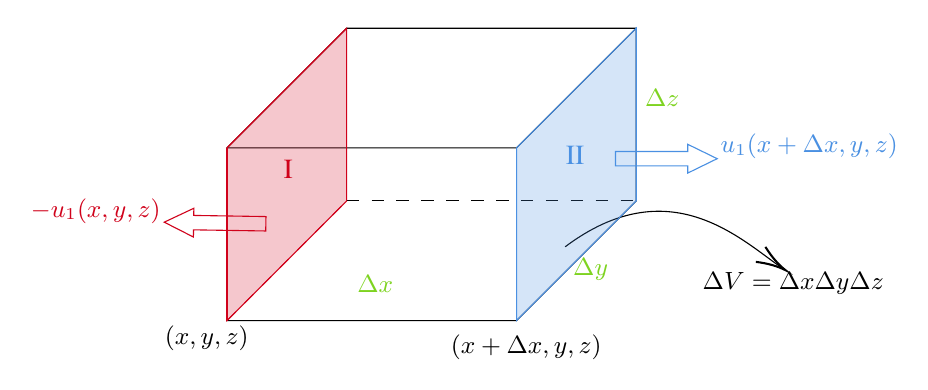
\begin{tikzpicture}[x=0.75pt,y=0.75pt,yscale=-1,xscale=1,scale=1.3]
    %uncomment if require: \path (0,155); %set diagram left start at 0, and has height of 155

    %Shape: Cube [id:dp6186431636735903] 
    \draw   (119.33,59.35) -- (163.68,15) -- (271,15) -- (271,79) -- (226.65,123.35) -- (119.33,123.35) -- cycle ; \draw   (271,15) -- (226.65,59.35) -- (119.33,59.35) ; \draw   (226.65,59.35) -- (226.65,123.35) ;
    %Straight Lines [id:da26318241804807796] 
    \draw [color={rgb, 255:red, 208; green, 2; blue, 27 }  ,draw opacity=1 ] [dash pattern={on 4.5pt off 4.5pt}]  (163.68,15) -- (163.68,79) ;
    %Straight Lines [id:da5928581432545683] 
    \draw  [dash pattern={on 4.5pt off 4.5pt}]  (163.67,79) -- (271,79) ;
    %Straight Lines [id:da8393161561837947] 
    \draw [color={rgb, 255:red, 208; green, 2; blue, 27 }  ,draw opacity=1 ] [dash pattern={on 4.5pt off 4.5pt}]  (119.33,123.35) -- (163.68,79) ;
    %Straight Lines [id:da08992921676399823] 
    \draw [color={rgb, 255:red, 208; green, 2; blue, 27 }  ,draw opacity=1 ]   (119.33,59.35) -- (163.68,15) ;
    %Straight Lines [id:da893341395756176] 
    \draw [color={rgb, 255:red, 208; green, 2; blue, 27 }  ,draw opacity=1 ]   (119.33,59.35) -- (119.33,123.35) ;
    %Curve Lines [id:da8206306595575221] 
    \draw    (244.67,96) .. controls (283.27,67.05) and (309.76,93.37) .. (324.75,103.63) ;
    \draw [shift={(326.33,104.68)}, rotate = 212.47] [color={rgb, 255:red, 0; green, 0; blue, 0 }  ][line width=0.75]    (10.93,-3.29) .. controls (6.95,-1.4) and (3.31,-0.3) .. (0,0) .. controls (3.31,0.3) and (6.95,1.4) .. (10.93,3.29)   ;
    %Shape: Polygon [id:ds9782874362859937] 
    \draw  [color={rgb, 255:red, 208; green, 2; blue, 27 }  ,draw opacity=1 ][fill={rgb, 255:red, 208; green, 2; blue, 27 }  ,fill opacity=0.22 ] (119.33,59.35) -- (146.83,31.85) -- (163.68,15) -- (163.68,79) -- (119.33,123.35) -- cycle ;
    %Shape: Polygon [id:ds6319731068332441] 
    \draw  [color={rgb, 255:red, 74; green, 144; blue, 226 }  ,draw opacity=1 ][fill={rgb, 255:red, 74; green, 144; blue, 226 }  ,fill opacity=0.23 ] (271,15) -- (271,79) -- (226.65,123.35) -- (226.65,59.35) -- cycle ;
    %Right Arrow [id:dp006127051123159699] 
    \draw  [color={rgb, 255:red, 74; green, 144; blue, 226 }  ,draw opacity=1 ] (263.33,60.68) -- (290.1,60.68) -- (290.1,58.02) -- (301,63.35) -- (290.1,68.68) -- (290.1,66.02) -- (263.33,66.02) -- cycle ;
    %Right Arrow [id:dp9412315249643457] 
    \draw  [color={rgb, 255:red, 208; green, 2; blue, 27 }  ,draw opacity=1 ] (133.69,90.14) -- (106.93,89.72) -- (106.89,92.38) -- (96.07,86.88) -- (107.05,81.72) -- (107.01,84.38) -- (133.78,84.8) -- cycle ;

    % Text Node
    \draw (139.33,63) node [anchor=north west][inner sep=0.75pt]  [color={rgb, 255:red, 208; green, 2; blue, 27 }  ,opacity=1 ] [align=left] {{\fontfamily{ptm}\selectfont I}};
    % Text Node
    \draw (244,57.67) node [anchor=north west][inner sep=0.75pt]  [color={rgb, 255:red, 74; green, 144; blue, 226 }  ,opacity=1 ] [align=left] {{\fontfamily{ptm}\selectfont II}};
    % Text Node
    \draw (95.33,124.4) node [anchor=north west][inner sep=0.75pt]  [font=\small]  {$( x,y,z)$};
    % Text Node
    \draw (201.33,127.73) node [anchor=north west][inner sep=0.75pt]  [font=\small]  {$( x+\Delta x,y,z)$};
    % Text Node
    \draw (166.67,105.73) node [anchor=north west][inner sep=0.75pt]  [font=\small,color={rgb, 255:red, 126; green, 211; blue, 33 }  ,opacity=1 ]  {$\Delta x$};
    % Text Node
    \draw (246.67,99.4) node [anchor=north west][inner sep=0.75pt]  [font=\small,color={rgb, 255:red, 126; green, 211; blue, 33 }  ,opacity=1 ]  {$\Delta y$};
    % Text Node
    \draw (273.33,36.73) node [anchor=north west][inner sep=0.75pt]  [font=\small,color={rgb, 255:red, 126; green, 211; blue, 33 }  ,opacity=1 ]  {$\Delta z$};
    % Text Node
    \draw (294.67,104.73) node [anchor=north west][inner sep=0.75pt]  [font=\small]  {$\Delta V=\Delta x\Delta y\Delta z$};
    % Text Node
    \draw (301.33,53.07) node [anchor=north west][inner sep=0.75pt]  [font=\small,color={rgb, 255:red, 74; green, 144; blue, 226 }  ,opacity=1 ]  {$u_{1}( x+\Delta x,y,z)$};
    % Text Node
    \draw (45.67,77.07) node [anchor=north west][inner sep=0.75pt]  [font=\small,color={rgb, 255:red, 208; green, 2; blue, 27 }  ,opacity=1 ]  {$-u_{1}( x,y,z)$};

    \end{tikzpicture}
    \end{center}

    Imagine the box with volume $\Delta V=\Delta x\Delta y\Delta z$, firstly consider faces $\rm \red I$ and $\rm \blue II$,
    the total flux {\it out of} faces $\rm \red I$ and $\rm \blue II$, as shown above, is: 
    \begin{align*}
        & [{\blue u_1(x+\Delta x,y,z)}-{\red u_1(x,y,z)}] \Delta y \Delta z\\
        = & \frac{[{\blue u_1(x+\Delta x,y,z)}-{\red u_1(x,y,z)}]}{\Delta x} \Delta x \Delta y \Delta z\\
        = & \frac{\pt u_1}{\pt x} \Delta x \Delta y \Delta z, \qquad {\rm( in\ the\ limit\ of\ } \Delta x\rightarrow 0)
    \end{align*}

    Similarly, the two faces in the $y-$ and $z-$ direction contribute 
    $$\frac{\pt u_2}{\pt y} \Delta x \Delta y \Delta z, \quad \frac{\pt u_3}{\pt z} \Delta x \Delta y \Delta z$$

    Hence net outward flux is: 
    $$\left(\frac{\pt u_1}{\pt x} + \frac{\pt u_2}{\pt y} + \frac{\pt u_3}{\pt z}\right)\cdot \Delta V$$
    Therefore outward flux {\it per unit volume} is $\nabla \cdot \uu$.



    \newpage
    \subsection{Interpretation of Curl}

    Curl is something related to rotation. Consider a small object flying in strong wind,
    where the speed and direction of wind can be treated as a vector field $\FF$. If the object 
    locates at position $\rr$, then its rotation has some relation with $\curl \FF$.

    Actually, the object will rotate about the direction $\nabla \times \FF(\rr)$(direction 
    is determined by right-hand rule), and with angular speed $\omega = \dfrac{1}{2} ||\nabla \times \FF(\rr)||$.
    \begin{center}
        \includegraphics[scale=0.13]{images/Ch15-curl-rotation.png}
    \end{center}

    {\blue The rest of this page prove the relation above.}

    Consider a disk in $xy-$plane, in $y$ direction, the differential velocity 
    {\it normal to }$\Delta x$ is: 
    $$u_2(x+\Delta x)-u_2(x)=\dfrac{\pt u_2}{\pt x}\Delta x$$
    \begin{center}
        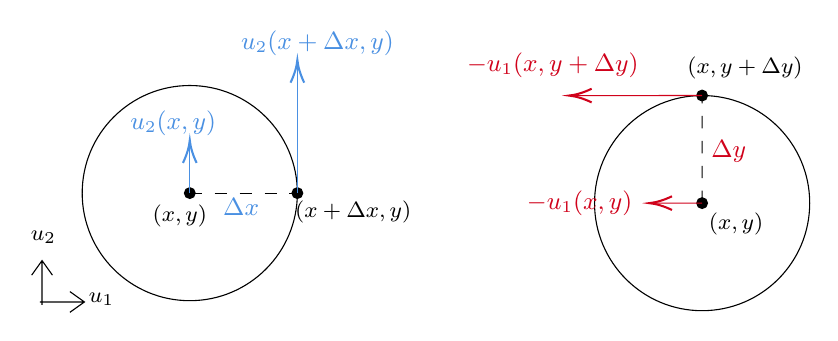
\begin{tikzpicture}[x=0.75pt,y=0.75pt,yscale=-1,xscale=1]
        %uncomment if require: \path (0,176); %set diagram left start at 0, and has height of 176

        %Shape: Circle [id:dp5225638015157492] 
        \draw   (51.33,105.83) .. controls (51.33,77.21) and (74.54,54) .. (103.17,54) .. controls (131.79,54) and (155,77.21) .. (155,105.83) .. controls (155,134.46) and (131.79,157.67) .. (103.17,157.67) .. controls (74.54,157.67) and (51.33,134.46) .. (51.33,105.83) -- cycle ;
        %Straight Lines [id:da39474822982601077] 
        \draw  [dash pattern={on 4.5pt off 4.5pt}]  (103.17,105.83) -- (155,105.83) ;
        \draw [shift={(155,105.83)}, rotate = 0] [color={rgb, 255:red, 0; green, 0; blue, 0 }  ][fill={rgb, 255:red, 0; green, 0; blue, 0 }  ][line width=0.75]      (0, 0) circle [x radius= 2.34, y radius= 2.34]   ;
        \draw [shift={(103.17,105.83)}, rotate = 0] [color={rgb, 255:red, 0; green, 0; blue, 0 }  ][fill={rgb, 255:red, 0; green, 0; blue, 0 }  ][line width=0.75]      (0, 0) circle [x radius= 2.34, y radius= 2.34]   ;
        %Straight Lines [id:da7639586630423449] 
        \draw [color={rgb, 255:red, 74; green, 144; blue, 226 }  ,draw opacity=1 ]   (103.17,105.83) -- (103.17,82.36) ;
        \draw [shift={(103.17,80.36)}, rotate = 450] [color={rgb, 255:red, 74; green, 144; blue, 226 }  ,draw opacity=1 ][line width=0.75]    (10.93,-3.29) .. controls (6.95,-1.4) and (3.31,-0.3) .. (0,0) .. controls (3.31,0.3) and (6.95,1.4) .. (10.93,3.29)   ;
        %Straight Lines [id:da012693447516093803] 
        \draw [color={rgb, 255:red, 74; green, 144; blue, 226 }  ,draw opacity=1 ]   (155,105.83) -- (155,43.69) ;
        \draw [shift={(155,41.69)}, rotate = 450] [color={rgb, 255:red, 74; green, 144; blue, 226 }  ,draw opacity=1 ][line width=0.75]    (10.93,-3.29) .. controls (6.95,-1.4) and (3.31,-0.3) .. (0,0) .. controls (3.31,0.3) and (6.95,1.4) .. (10.93,3.29)   ;
        %Shape: Axis 2D [id:dp8368267344724862] 
        \draw  (31,158.28) -- (52.4,158.28)(31.99,138.36) -- (31.99,159.69) (45.4,153.28) -- (52.4,158.28) -- (45.4,163.28) (26.99,145.36) -- (31.99,138.36) -- (36.99,145.36)  ;
        %Shape: Circle [id:dp5099823978536693] 
        \draw   (350.03,162.49) .. controls (321.4,162.5) and (298.19,139.31) .. (298.18,110.68) .. controls (298.17,82.05) and (321.37,58.84) .. (349.99,58.83) .. controls (378.62,58.82) and (401.83,82.02) .. (401.84,110.64) .. controls (401.85,139.27) and (378.66,162.48) .. (350.03,162.49) -- cycle ;
        %Straight Lines [id:da7840728663323955] 
        \draw  [dash pattern={on 4.5pt off 4.5pt}]  (350.01,110.66) -- (349.99,58.83) ;
        \draw [shift={(349.99,58.83)}, rotate = 269.98] [color={rgb, 255:red, 0; green, 0; blue, 0 }  ][fill={rgb, 255:red, 0; green, 0; blue, 0 }  ][line width=0.75]      (0, 0) circle [x radius= 2.34, y radius= 2.34]   ;
        \draw [shift={(350.01,110.66)}, rotate = 269.98] [color={rgb, 255:red, 0; green, 0; blue, 0 }  ][fill={rgb, 255:red, 0; green, 0; blue, 0 }  ][line width=0.75]      (0, 0) circle [x radius= 2.34, y radius= 2.34]   ;
        %Straight Lines [id:da7720976544639997] 
        \draw [color={rgb, 255:red, 208; green, 2; blue, 27 }  ,draw opacity=1 ]   (350.01,110.66) -- (326.54,110.67) ;
        \draw [shift={(324.54,110.67)}, rotate = 359.98] [color={rgb, 255:red, 208; green, 2; blue, 27 }  ,draw opacity=1 ][line width=0.75]    (10.93,-3.29) .. controls (6.95,-1.4) and (3.31,-0.3) .. (0,0) .. controls (3.31,0.3) and (6.95,1.4) .. (10.93,3.29)   ;
        %Straight Lines [id:da7249887830259147] 
        \draw [color={rgb, 255:red, 208; green, 2; blue, 27 }  ,draw opacity=1 ]   (349.99,58.83) -- (287.85,58.85) ;
        \draw [shift={(285.85,58.85)}, rotate = 359.98] [color={rgb, 255:red, 208; green, 2; blue, 27 }  ,draw opacity=1 ][line width=0.75]    (10.93,-3.29) .. controls (6.95,-1.4) and (3.31,-0.3) .. (0,0) .. controls (3.31,0.3) and (6.95,1.4) .. (10.93,3.29)   ;

        % Text Node
        \draw (118,107.07) node [anchor=north west][inner sep=0.75pt]  [font=\small,color={rgb, 255:red, 74; green, 144; blue, 226 }  ,opacity=1 ]  {$\Delta x$};
        % Text Node
        \draw (84,110.4) node [anchor=north west][inner sep=0.75pt]  [font=\footnotesize]  {$( x,y)$};
        % Text Node
        \draw (152.67,108.4) node [anchor=north west][inner sep=0.75pt]  [font=\footnotesize]  {$( x+\Delta x,y)$};
        % Text Node
        \draw (73.33,65.07) node [anchor=north west][inner sep=0.75pt]  [font=\small,color={rgb, 255:red, 74; green, 144; blue, 226 }  ,opacity=1 ]  {$u_{2}( x,y)$};
        % Text Node
        \draw (126.67,26.4) node [anchor=north west][inner sep=0.75pt]  [font=\small,color={rgb, 255:red, 74; green, 144; blue, 226 }  ,opacity=1 ]  {$u_{2}( x+\Delta x,y)$};
        % Text Node
        \draw (53.33,152.73) node [anchor=north west][inner sep=0.75pt]  [font=\footnotesize]  {$u_{1}$};
        % Text Node
        \draw (25.33,122.73) node [anchor=north west][inner sep=0.75pt]  [font=\footnotesize]  {$u_{2}$};
        % Text Node
        \draw (353.17,79.23) node [anchor=north west][inner sep=0.75pt]  [font=\small,color={rgb, 255:red, 208; green, 2; blue, 27 }  ,opacity=1 ]  {$\Delta y$};
        % Text Node
        \draw (352.01,114.06) node [anchor=north west][inner sep=0.75pt]  [font=\footnotesize]  {$( x,y)$};
        % Text Node
        \draw (341.65,39.06) node [anchor=north west][inner sep=0.75pt]  [font=\footnotesize]  {$( x,y+\Delta y)$};
        % Text Node
        \draw (264.35,103.41) node [anchor=north west][inner sep=0.75pt]  [font=\small,color={rgb, 255:red, 208; green, 2; blue, 27 }  ,opacity=1 ]  {$-u_{1}( x,y)$};
        % Text Node
        \draw (235.49,36.92) node [anchor=north west][inner sep=0.75pt]  [font=\small,color={rgb, 255:red, 208; green, 2; blue, 27 }  ,opacity=1 ]  {$-u_{1}( x,y+\Delta y)$};
        \end{tikzpicture}

    \end{center}
    Recall that $v=\omega r$, so the angular velocity is $\omega_1 = \dfrac{\pt u_2}{\pt x}$

    Similarly, in the $y-$direction, (notice the negative sign)
    $$-u_1(x,y+\Delta y)+u_1(x,y)=-\dfrac{\pt u_1}{\pt y}\Delta y,\qquad 
    \omega_2 = -\dfrac{\pt u_1}{\pt y}$$

    Thus the {\it averaged angular velocity} is: $\disp \omega = \frac{1}{2} 
    \left(\frac{\pt u_2}{\pt x} - \frac{\pt u_1}{\pt y}\right)$

    The curl of this vector field is: 
    $$
    \operatorname{curl} \mathbf{F}=\nabla \times \mathbf{F}=\left|\begin{array}{ccc}
    \mathbf{i} & \mathbf{j} & \mathbf{k} \\
    \dfrac{\partial}{\partial x} & \dfrac{\partial}{\partial y} & \dfrac{\partial}{\partial z} \\
    u_1 & u_2 & 0
    \end{array}\right|= \left(\frac{\pt u_2}{\pt x} - \frac{\pt u_1}{\pt y}\right)\kk =2\omega \kk
    $$
    Thus prove the result.


    \vspace{0.5in}
    {\blue Below example is used to explain the meaning of curl, it's the same example in intro.}

    \eg Assume a vector field: ${\bf F}(x,y)=\dfrac{y\ii -x\jj}{\sqrt{x^2+y^2}}$.

    \sol
    \begin{align*}
        {\vec{\omega}} &= \nabla \times \FF = \left|\begin{array}{ccc}
            \ii & \jj & \kk \\ \dfrac{\partial}{\partial x} & \dfrac{\partial}{\partial y} & \dfrac{\partial}{\partial z} \\
            \dfrac{y}{\sqrt{x^2+y^2}} & \dfrac{-x}{\sqrt{x^2+y^2}} & 0
        \end{array} \right|\\
        &= \left[ -\dfrac{\pt}{\pt x}\left( \dfrac{x}{\sqrt{x^2+y^2}} \right)
                -\dfrac{\pt}{\pt y}\left( \dfrac{y}{\sqrt{x^2+y^2}}\right) \right] \kk \\
        &= {\bf 0}   
    \end{align*}

    Consider a small object in the vector field, it doesn't rotate(since $\curl \FF={\bf 0}$ everywhere),
    it just move in circular, along the vector field.

    \begin{center}
        \includegraphics[scale=0.4]{images/Ch15-ex1.2.png}
    \end{center}

    \newpage
    {\blue This definition is optional.}
    
    {\bf Laplacian Operator}
    $$
    \begin{aligned}
    \nabla^{2} &=\nabla \cdot \nabla=\left(\mathbf{i} \frac{\partial}{\partial x}+\mathbf{j} \frac{\partial}{\partial y}+\mathbf{k} \frac{\partial}{\partial z}\right) \cdot\left(\mathbf{i} \frac{\partial}{\partial x}+\mathbf{j} \frac{\partial}{\partial y}+\mathbf{k} \frac{\partial}{\partial z}\right) \\
    &=\frac{\partial^{2}}{\partial x^{2}}+\frac{\partial^{2}}{\partial y^{2}}+\frac{\partial^{2}}{\partial z^{2}}
    \end{aligned}
    $$
    $\nabla^{2}$ is a {\bf scalar} differential operator. Note that
    $$
    \begin{aligned}
    \nabla^{2} f &=\frac{\partial^{2} f}{\partial x^{2}}+\frac{\partial^{2} f}{\partial y^{2}}+\frac{\partial^{2} f}{\partial z^{2}} \\
    \nabla^{2} \mathbf{F} &=\nabla^{2} F_{1} \mathbf{i}+\nabla^{2} F_{2} \mathbf{j}+\nabla^{2} F_{3} \mathbf{k}
    \end{aligned}
    $$

    \newpage
    \subsection{Vector differential identities}
    Let $\phi, \psi$ are scalar fields and $\mathbf{F}$ and $\mathbf{G}$ are vector fields, then

    (a) $\nabla(\phi \psi)=\phi \nabla \psi+\psi \nabla \phi$

    (b) $\nabla \cdot(\phi \mathbf{F})=\nabla \phi \cdot \mathbf{F}+\phi(\nabla \cdot \mathbf{F})$

    (c) $\nabla \times(\phi \mathbf{F})=\nabla \phi \times \mathbf{F}+\phi(\nabla \times \mathbf{F})$

    (d) $\nabla \cdot(\mathbf{F} \times \mathbf{G})=(\nabla \times \mathbf{F}) \cdot \mathbf{G}-\mathbf{F} \cdot(\nabla \times \mathbf{G})$
    
    (e) $\nabla \cdot(\nabla \times \mathbf{F})=0$
    
    (f) $\nabla \times(\nabla \phi)=0$
    
    (g) $\nabla \times(\nabla \times \mathbf{F})=\nabla(\nabla \cdot \mathbf{F})-\nabla^{2} \mathbf{F}$

    \vspace{0.2in}
    {\bf [Proof.]}



    \newpage
    \section{Line Integral}
    {\bf Motivation:} given a rope(parametrized space curve) $\rr(t), a\le t\le b$, if the density at 
    point $(x,y,z)$ is given by function $\rho =f(x,y,z)$, we want to find the mass of this rope.
    $$\int_a^b f(x,y,z)\ ds=\int_C f(x,y,z)\ ds$$

    Recall when we computing arc length in Chapter 11, we knew that: 
    $$ds=||\rr'(t)|| dt$$

    Therefore, to calculate line integral $\disp \int_C f(x,y,z)\ ds$, we only need to know: 
    \begin{enumerate}
        \item $f(x,y,z)$
        \item Region $C:\ \rr(t)=(x(t), y(t), z(t)),\ a\le t\le b$
    \end{enumerate}

    {\blue This example shows how to find line integral.}

    \eg Find $\disp \int_{C} x y^{4} d s, C$ is the right half of the circle $x^{2}+y^{2}=16$.

    \sol In order to do this integral, we need the parametric form of the path $C$.
    Let $x=4\cos t, t=4\sin t$, the right half of the circle means $t \in[-\pi / 2, \pi / 2]$.

    Hence the parametric equation of the curve $C$ is
    4
    $\mathbf{r}(t)=4 \cos t \mathbf{i}+4 \sin t \mathbf{j}$ with $t \in[-\pi / 2, \pi / 2]$, then
    $$\mathbf{r}^{\prime}(t)=-4 \sin t \mathbf{i}+4 \cos t \mathbf{j} \quad \text { and } \quad\left\|\mathbf{r}^{\prime}(t)\right\|=4$$

    Thus with $ds=||\rr'(t)|| dt$,
    $$\int_{C} x y^{4} d s =\int_{-\pi / 2}^{\pi / 2} f(\mathbf{r})\left\|\mathbf{r}^{\prime}(t)\right\| d t=
    \int_{-\pi / 2}^{\pi / 2}\left[4^{5} \cos t \sin ^{4} t\right](4) d t =\frac{2\cdot 4^6}{5}$$

    {\blue Note that there are infinitely many ways to parametrize the curve $C$, }
    for example, if we had parameterized $C$ as
    $$\mathbf{r}(t)=\sqrt{16-t^{2}} \mathbf{i}+t \mathbf{j} \quad \text { where } \quad-4 \leqslant t \leqslant 4$$
    Then
    $$\mathbf{r}^{\prime}(t) =-\frac{t}{\sqrt{16-t^{2}}} \mathbf{i}+\mathbf{j}, \qquad
    \left\|\mathbf{r}^{\prime}(t)\right\| =\sqrt{\frac{16}{16-t^{2}}} $$

    $$ \int_{C} x y^{4} d s =\int_{C} f(\mathbf{r})\left\|\mathbf{r}^{\prime}(t)\right\| d t
    =\int_{-4}^{4} \sqrt{16-t^{2}} \times t^{4} \times \sqrt{\frac{16}{16-t^{2}}} d t=\frac{2\cdot 4^6}{5}$$
    Thus the line integral is {\it \blue independent of parametrization} of the curve C.

    So far, we have been doing integration w.r.t. $s$, but we can also carry the integration w.r.t. $x$,
    $$\int_C f(\rr(t))\ dx$$

    \vspace{0.3in}
    {\blue This example shows how to integrate w.r.t. $x,y,z$}

    \eg $f(\rr(t))=f(x,y,z)=xy+z$, $C: \rr(t)=(x(t), y(t), z(t)) = (t^2, t^3, t), 0\le t\le 1$

    \sol Since $dx=2t\ dt,\ dy=3t^2\ dt,\ dz=dt$,
    \begin{align*}
        \int_C f(\rr(t))\ {\blue dx} &= \int_0^1 (t^2\cdot t^3+t)(2t)\ dt=\int_0^1 (2t^6-2t^2)\ dt=\cdots\\
        \int_C f(\rr(t))\ {\blue dy} &= \int_0^1 (t^5+t)(3t^2)\ dt=\cdots\\
        \int_C f(\rr(t))\ {\blue dz} &= \int_0^1 (t^5+t)\ dt=\cdots
    \end{align*}

    \vspace{0.8in}
    But why are we doing this? Consider given $f(\rr(t))$ and $C: \rr(t)$, we integrate w.r.t. $x,y,z$, respectively: 
    $$\int_C f(\rr(t))\ dx\qquad \int_C g(\rr(t))\ dy\qquad \int_C h(\rr(t))\ dz$$
    The summation of above three gives: 
    \begin{align*}
        & \int_C \left[f(\rr(t))\ dx + g(\rr(t))\ dy + h(\rr(t))\ dz\right]\\
        =& \int_C (f, g, h) \cdot (dx, dy, dz)\\
        =& \boxed{\int_C \FF \cdot d\rr}
    \end{align*}
    where $\FF(\rr)=\left(f(\rr), g(\rr), h(\rr)\right)$ is the given vector field.


    \newpage
    {\blue The following two examples shows usage of integration w.r.t. $x, y, z$.}

    \eg $\disp \int_{C} x y d x+(x-y) d y, C$ consists of line segments from $(0,0)$ to $(2,0)$ and from $(2,0)$ to $(3,2)$.
    \begin{center}
        \includegraphics[scale=0.38]{images/Ch15-wrt-eg1.png}
    \end{center}

    \sol We need the parametric function of $C_1$ and $C_2$, they are straight lines.
    Recall in Chapter 10 we know the parameterized curve of straight lines can be written as: 
    $$\rr(t)=(1-t)\rr_1+t\rr_2, \ 0\le t\le 1$$

    Hence 
    \begin{align*}
        C1: \ \rr(t) &= (1-t)(0, 0) + t(2, 0) = (2t, 0) = (x(t), y(t)),\ 0\le t\le 1\\
        C2: \ \rr(t) &= (1-t)(2, 0) + t(3, 2) = (2+t, 2t) = (x(t), y(t)),\ 0\le t\le 1
    \end{align*}
    Thus the integration is: 
    \begin{align*}
        \int_C xydx+(x-y)dy &= \int_{C_1} xydx+(x-y)dy + \int_{C_2} xydx+(x-y)dy\\
                    &= \int_0^1 (2t)(0) 2dt+(2t-0)(0) +\int_0^1 (2+t)(2t)dt + (2+t-2t) 2dt\\
                    &= \int_0^1 (4t+2t^2+2+t-2t) dt =\cdots
    \end{align*}
    {\blue Notice that: } if $\FF(\rr)=(xy, x-y)$, and $\rr_1=(2t, 0), \rr_2=(2+t,2t)$, 
    the result above is exactly 
    $$\int_{C_1} \FF\cdot d\rr + \int_{C_2} \FF\cdot d\rr$$

    {\blue Again, there are many ways to parameterized the curve, } for example,

    $C_{1}: (x, 0),\  0 \le x \le 2, \qquad C_{2}: (x, 2x-4),\  2 \le x \le 3 .$ 
    
    Then
    \begin{align*}
        \int_{C} x y d x+(x-y) d y 
        &=\int_{C_{1}}[x y d x+(x-y) d y]+\int_{C_{2}}[x y d x+(x-y) d y] \\
        &=\int_{0}^{2} 0 d x+\int_{2}^{3}\left(2 x^{2}-4 x\right) d x+\int_{2}^{3}(-x+4) 2 d x = \cdots
    \end{align*}

    \newpage
    \eg 
    \begin{center}
        \includegraphics[scale=0.52]{images/Ch15-wrt-eg2.png}
    \end{center}

    \newpage
    \section{Line Integration in Vector Fields}
    We have talked so much about line integration above. However, this Chapter is called ``Vector Field'',
    so how does line integration relate to vector field?

    {\blue The following two examples show that sometimes the line integral depends on path,
    while sometimes it does not.}

    \eg Find $\disp \int_{C} \mathbf{F} \cdot d \mathbf{r}$, where $\mathbf{F}(x, y)=e^{x-1} \mathbf{i}+x y \mathbf{j}$ 
    and $C$ is given by

    (a) $\mathbf{r}(t)=t^{2} \mathbf{i}+t^{3} \mathbf{j} ; \quad 0 \leqslant t \leqslant 1$.\\
    (b) $\mathbf{r}(t)=t \mathbf{i}+t \mathbf{j} ; \quad 0 \leqslant t \leqslant 1 .$

    \sol 

    (a)
    $$\begin{aligned}
    \int_{C} \mathbf{F} \cdot d \mathbf{r} &=\int_{0}^{1} \mathbf{F}(\mathbf{r}(t)) \cdot \mathbf{r}^{\prime}(t) d t=\int_{0}^{1} \mathbf{F}\left(t^{2}, t^{3}\right) \cdot \mathbf{r}^{\prime}(t) d t \\
    &=\int_{0}^{1}\left(e^{t^{2}-1} \mathbf{i}+t^{5} \mathbf{j}\right) \cdot\left(2 t \mathbf{i}+3 t^{2} \mathbf{j}\right) d t \\
    &=\int_{0}^{1}\left(2 t e^{t^{2}-1}+3 t^{7}\right) d t =\left[e^{t^{2}-1}+\frac{3}{8} t^{8}\right]_{0}^{1}=\frac{11}{8}-\frac{1}{e}
    \end{aligned}$$

    (b)
    $$\begin{aligned}
    \int_{C} \mathbf{F} \cdot d \mathbf{r} &=\int_{0}^{1} \mathbf{F}(\mathbf{r}(t)) \cdot \mathbf{r}^{\prime}(t) d t=\int_{0}^{1} \mathbf{F}(t, t) \cdot \mathbf{r}^{\prime}(t) d t \\
    &=\int_{0}^{1}\left(e^{t-1} \mathbf{i}+t^{2} \mathbf{j}\right) \cdot(\mathbf{i}+\mathbf{j}) d t \\
    &=\int_{0}^{1}\left(e^{t-1}+t^{2}\right) d t =\frac{4}{3}-\frac{1}{e}
    \end{aligned}$$

    {\blue Note that the line integral depends on the path.}
    
    \vspace{0.2in}
    \eg Find $\disp \int_{C} \mathbf{F} \cdot d \mathbf{r}$, where $\mathbf{F}(x, y)=y \mathbf{i}+x \mathbf{j}$ and $C$ is given by
    
    (a) $\mathbf{r}(t)=t \mathbf{i}+t \mathbf{j} ; \quad 0 \leqslant t \leqslant 1$.\hspace{0.2in}
    (b) $\mathbf{r}(t)=t \mathbf{i}+t^{2} \mathbf{j} ; \quad 0 \leqslant t \leqslant 1$\hspace{0.2in}
    (c) $\mathbf{r}(t)=t \mathbf{i}+t^{3} \mathbf{j} ; \quad 0 \leqslant t \leqslant 1$.

    \sol

    (a) $\disp \int_{C} \mathbf{F} \cdot d \mathbf{r}=\int_{0}^{1}(t \mathbf{i}+t \mathbf{j}) \cdot(\mathbf{i}+\mathbf{j}) d t=\int_{0}^{1} 2 t d t=1$
    
    (b) $\disp \int_{C} \mathbf{F} \cdot d \mathbf{r}=\int_{0}^{1}\left(t^{2} \mathbf{i}+t \mathbf{j}\right) \cdot(\mathbf{i}+2 \mathbf{j}) d t=\int_{0}^{1} 3 t^{2} d t=1$
    
    (c) $\disp \int_{C} \mathbf{F} \cdot d \mathbf{r}=\int_{0}^{1}\left(t^{3} \mathbf{i}+t \mathbf{j}\right) \cdot\left(\mathbf{i}+3 t^{2} \mathbf{j}\right) d t=\int_{0}^{1} 4 t^{3} d t=1$

    {\blue Note that this integral does not depend on path.}

    \newpage
    \section{Conservative Vector Fields}

    {\blue So why different vector field cause different results in above examples?}
    
    Recall that if $\disp \int_a^b f(x) dx=F(b)-F(a)$ (that the integral only depends on the 
    {\it end points}) only if {\it anti-derivative } exists, otherwise, we cannot integrate it
    and hence cannot express it only with end points.

    For example, $\disp \int_1^2 e^x dx = e^2-e^1$, but for $\disp \int_1^2 e^{x^2} dx$,
    we cannot find it.

    \vspace{0.3in}
    Similarly, if $\FF(\rr)=f(\rr)\ii +g(\rr)\jj +h(\rr)\kk$ is the gradient of a function 
    $\phi(\rr)$ on $S$, i.e.,
    $$\FF(\rr)=\nabla \phi(\mathbf{r}) \quad \Rightarrow \quad 
    f(\mathbf{r})=\frac{\partial \phi}{\partial x}, \quad g(\mathbf{r})=\frac{\partial \phi}{\partial y} \quad 
    \text { and } \quad h(\mathbf{r})=\frac{\partial \phi}{\partial z}$$

    In that case, we say $\mathbf{F}(\mathbf{r})$ is a {\bf conservative field} and $\phi$ is a 
    {\it (scaler) potential function} of $\FF$ on $S$.
    
    Then
    $$\begin{aligned}
    \int_{C} \mathbf{F}(\mathbf{r}) \cdot d \mathbf{r} &=\int_{a}^{b} \nabla \phi(\mathbf{r}(t)) \cdot \mathbf{r}^{\prime}(t) d t \\
    &=\int_{a}^{b}\left(\frac{\partial \phi}{\partial x} \frac{d x}{d t}+\frac{\partial \phi}{\partial y} \frac{d y}{d t}+\frac{\partial \phi}{\partial z} \frac{d z}{d t}\right) d t \\
    &=\int_{a}^{b} \frac{d \phi}{d t} d t=\phi(x(b), y(b), z(b))-\phi(x(a), y(a), z(a)) \\
    &=\phi(\mathbf{r}(b))-\phi(\mathbf{r}(a))
    \end{aligned}$$

    This depends only {\it on the endpoints} $\mathbf{r}(b)$ and $\mathbf{r}(a)$, not on the curve $C.$

    \vspace{0.5in}
    This can also be expressed in circular integration, $\disp \int_C \FF\cdot d\rr$ is {\it independent} of 
    path in $S$ if and only if $\disp \oint_C \FF\cdot d\rr =0$ for {\it every closed path} $C$ in $S$.
    Since if the integration depends only on end points, then integrate from $a$ to $b$ and then from $b$
    back to $a$ will certainly gives result 0.
    \begin{center}
        \includegraphics[scale=0.4]{images/Ch15-circular-integ.png}
    \end{center}
    $$\oint_{C} \FF \cdot d \rr =\int_{C_{1}} \FF \cdot d \rr+\int_{C_{2}} \mathbf{F} \cdot d \mathbf{r} 
    =\int_{C_{1}} \mathbf{F} \cdot d \mathbf{r}-\int_{-C_{2}} \mathbf{F} \cdot d \mathbf{r}=0 $$

    \newpage
    {\blue How to determine whether a vector field is {\it conservative} or not?}

    A continuously vector field $\mathbf{F}$ defined in a {\bf simply-connected domain} $S$ is conservative 
    if and only if, it possesses {\it any one} of the following properties.
    
    (i) It is the gradient of a scalar function, $\mathbf{F}(\mathbf{r})=\nabla \phi(\mathbf{r})$.
    
    (ii) Its line integral along any regular curve extending from a point $P$ to a point $Q$ is independent of the path.
    $$
    \int_{C_{1}} \mathbf{F} \cdot d \mathbf{r}=\int_{C_{2}} \mathbf{F} \cdot d \mathbf{r}=\int_{C_{3}} \mathbf{F} \cdot d \mathbf{r}=\cdots
    $$
    (iii) Its line integral around any regular closed curved is zero, i.e. $\disp \oint_{C} \mathbf{F} \cdot d \mathbf{r}=0$.

    (iv) $\nabla \times \FF ={\bf 0}$. (since $\nabla \times (\nabla\times \phi)={\bf 0}$)

    {\blue Note that $(i)\Rightarrow (ii)\Rightarrow (iii)$, and it's trivial that $(iii)\Rightarrow (ii)$}

    \vspace{0.2in}
    {\bf For $(ii)\Rightarrow (i)$}, this can be proved only if $\FF$ us continuous on an {\it open connected region}.
    Proof is not required here.

    {\bf For $(iv)$}, this is a {\bf necessary} condition for the existence of a potential function $\phi$,
    in other words, this is {\bf not sufficient}, we also need to guarantee that the domain $S$ 
    must be {\bf open and simply connected.}

    \vspace{0.3in}
    What is {\bf open and simply-connected} region?

    Firstly, it must be {\it connected}, it cannot be divided into two parts that are separate. For example,

    (1) $\disp \FF(\rr)=\left(\frac{x}{x^2+y^2+z-1}, \frac{y}{x^2+y^2+z-1}, \frac{z^2}{x^2+y^2+z-1}\right)$
    is defined on $\mathbb{R}^3\backslash \{x^2+y^2+z=1\}$. This is not connected, because the region 
    is divided into two parts by a ``rice bowl''.

    (2) Also, $\mathbb{R}^3\backslash \{x^2+y^2+z^2=1\}$ is not connected, because the region 
    is divided into two parts by a ball shell.

    Then, for {\it any curve} inside the region, if {\it at least one surface} inside the region
    with the curve {\it as boundary}
    does not have a hole on it, then the region is simply-connected. For example,

    (1) $\mathbb{R}^2\backslash \{(0,0)\}$ is not simply-connected. Consider any curve surround the origin,
    the only surface that with the curve as boundary is the ``disk'' bounded by the curve, and unfortunately 
    it has a hole in the middle.

    (2) $\mathbb{R}^3\backslash \{(0,0,0)\}$ is simply-connected. For any curve inside the region, even if 
    you choose a curve on $xy$-plane and contains $(0,0,0)$, we can easily find a surface bounded by the 
    curve that does not contain the origin, for example a downside ``rice bowl''.

    (3) $\mathbb{R}^3\backslash \{x=y=0\}$ is not simply-connected. For example, if we choose a circle on 
    $xy-$plane, like $x^2+y^2=1$, then {\it any} surface bounded by the curve must through $z-$axis,
    and since we've removed the $z-$axis, all those surfaces always have a hole on it.

    (4) A donut is not simply-connected, we can choose any curve that surround the middle ``hole''.


    {\blue This example shows how to find potential for a conservative vector field.}

    \eg Determine whether or not $\mathbf{F}(x, y)=(2 x-3 y) \mathbf{i}+(2 y-3 x) \mathbf{j}$ 
    is a conservative vector field. If it is, find a function $\phi$ such that $\mathbf{F}=\nabla \phi$.

    \sol Notice that the curl of $\FF$:
    $$\nabla \times \FF=\left|\begin{array}{ccc}
        \ii & \jj & \kk \\
        \dfrac{\pt}{\pt x} & \dfrac{\pt}{\pt x} & 0\\
        2x-3y & 2y-3x & 0
    \end{array} \right|={\bf 0}$$
    And, $\FF(x,y)$ is defined in $\mathbb{R}^2$, which is {\bf open and simply-connected} domain.
    Therefore, $\FF$ is conservative and $\FF=\nabla \phi$ for some potential function $\phi$.

    To find $f$,
    \begin{align*}
        \frac{\pt \phi}{\pt x} &= 2x-3y\qquad (1)\\
        \frac{\pt \phi}{\pt y} &= 2y-3x\qquad (2)
    \end{align*}
    For (1), integrate w.r.t. $x$, $\phi(x,y)=x^2-3xy+g(y)$, differentiate it w.r.t. $y$,
    $\disp \frac{\pt \phi}{\pt y}=0-3x+g'(y)$.

    Compare this equation with (2), we have $g'(y)=2y \Rightarrow g(y)=y^2+C$

    Therefore $$\phi(x, y)=x^2-3xy+y^2+C.$$

    \newpage
    {\blue This example shows $\curl \FF={\bf 0}$ is not sufficient for $\FF$ to be conservative.}

    \eg Let $\disp \mathbf{F}(x, y)=\frac{-y \mathbf{i}+x \mathbf{j}}{x^{2}+y^{2}}=f(x, y) \mathbf{i}+g(x, y) \mathbf{j}$ (see also Ex. 1.2).
    
    (a) Show that $\disp \frac{\partial f}{\partial y}=\frac{\partial g}{\partial x}$.

    (b) Show that $\disp \int_{C} \mathbf{F} \cdot d \mathbf{r}$ is not independent of path.
    
    \sol (a)$$\frac{\partial f}{\partial y}=\frac{y^{2}-x^{2}}{\left(x^{2}+y^{2}\right)^{2}}=\frac{\partial g}{\partial x}$$

    (b) Notice $\FF$ is defined on $\mathbb{R}^2\backslash \{{\bf 0}\}$, so it is not conservative.
    To show that it is dependent of path, we only need to given an counterexample. Consider on these two paths:
    \begin{center}
        \includegraphics[scale=0.4]{images/Ch15-ex2.3.png}
    \end{center}
    $C_{1}: \quad x=\cos \theta, \quad y=\sin \theta$, with $\theta = 0$ to $\theta = \pi$\\
    $C_{2}: \quad x=\cos \theta, \quad y=\sin \theta$, with $\theta = 2\pi$ to $\theta = \pi$

    $$\int_{C_{1}} \mathbf{F} \cdot d \mathbf{r}=\int_{0}^{\pi}(-\sin \theta, \cos \theta) \cdot(-\sin \theta, \cos \theta) d \theta=\int_{0}^{\pi} d \theta=\pi$$
    $$\int_{C_{2}} \mathbf{F} \cdot d \mathbf{r}=\int_{2 \pi}^{\pi} d \theta=-\pi \neq \int_{C_{1}} \mathbf{F} \cdot d \mathbf{r}$$

    Therefore, $\disp \int_{C} \mathbf{F} \cdot d \mathbf{r}$ is not independent of path.

    \vspace{0.3in}
    {\blue But if $\FF$ is defined on $x>0$, it will become a conservative field. ($x>0$ is open and simply-connected.)}


    \newpage
    {\blue In summary, to find a line integral, you have following methods:}
    \begin{enumerate}
        \item Carry out the integration directly: 
        $$\int_C \FF\cdot d\rr=\int_z^b g(t) dt\cdots$$
        \item If $\nabla \times \FF \ne {\bf 0}$, nothing you can do, except for 
        carrying the integration as above.
        \item If $\nabla \times \FF = {\bf 0}$, there are two simpler ways:
        \begin{enumerate}
            \item Find $\phi$ such that $\FF =\nabla \phi$, then 
            $$\int_C \FF \cdot d\rr=\phi (\rr(b))-\phi (\rr(a))$$
            \item Carry the integration along a straight line path, i.e. 
            $$\rr(t)=(1-t)\rr_1+t\rr_2,\ 0\le t\le 1$$
        \end{enumerate}
    \end{enumerate}

    \newpage
    {\blue This is a past final question in year 1994.}

    \eg For what values of $b$ and $c$ will
    $$\mathbf{F}(x, y, z)=\left(y^{2}+2 c z x\right) \mathbf{i}+y(b x+c z) \mathbf{j}+\left(y^{2}+c x^{2}\right) \mathbf{k}$$
    have potential functions? For each pair of these values of $b$ and $c$, find a potential function for $\mathbf{F}$.

    \sol 
    For $\mathbf{F}(\mathbf{r})$ to have a potential function, iff $\nabla \times \mathbf{F}(\mathbf{r})=\mathbf{0}$.
    $$\nabla \times \mathbf{F}=\left|\begin{array}{ccc}
        \mathbf{i} & \mathbf{i} & \mathbf{k} \\
        \dfrac{\partial}{\partial x} & \dfrac{\partial}{\partial y} & \dfrac{\partial}{\partial z} \\
        y^{2}+2 c z x & y(b x+c z) & y^{2}+c x^{2}
    \end{array}\right|$$

    For the $\ii$ component, $2 y=y c \quad \Rightarrow \quad c=2$

    For the $\jj$ component, $2 c x=2 c x \quad \Rightarrow \quad c \text { cannot be determined. }$
    
    For the $\kk$ component, $b y=2 y \quad \Rightarrow \quad b=2$

    $\therefore b=2$ and $c=2 .$ In the case, we have
    $$\mathbf{F}(\mathbf{r})=\left(y^{2}+4 z x\right) \mathbf{i}+y(2 x+2 z) \mathbf{j}+\left(y^{2}+2 x^{2}\right) \mathbf{k}=\nabla \phi$$
    
    Therefore
    $$\begin{aligned}
    &\frac{\partial \phi}{\partial x}=y^{2}+4 z x \qquad (1)\\
    &\frac{\partial \phi}{\partial y}=2 x y+2 y z \qquad (2)\\
    &\frac{\partial \phi}{\partial z}=y^{2}+2 x^{2} \qquad (3)
    \end{aligned}$$
    From $(1)$, we have
    $$\begin{aligned}
    \phi(x, y, z) &=x y^{2}+2 x^{2} z+p(y, z) \qquad (4)\\
    \phi_{y}(x, y, z) &=2 x y+p_{y}(y, z) \qquad (5)
    \end{aligned}$$
    Comparing $(2)$ and $(5)$, we have $p_{y}(y, z)=2 y z \Rightarrow p(y, z)=y^{2} z+q(z) .$ From $(4)$, we have
    $$\begin{aligned}
    \phi(x, y, z) &=x y^{2}+2 x^{2} z+y^{2} z+q(z) \qquad(6)\\
    \phi_{z}(x, y, z) &=2 x^{2}+y^{2}+q^{\prime}(z) \qquad(7)
    \end{aligned}$$
    Comparing $(7)$ and $(3)$, we have $q^{\prime}(z)=0 \quad \Rightarrow \quad q(z)=k$ (constant).
    $$\therefore \quad \phi(x, y, z)=x y^{2}+2 x^{2} z+y^{2} z+k$$

    \newpage
    \section{Surface Integrals of Vector Fields}
    \subsection{Surface Integrals}

    {\blue Recall in Chapter 14, we discussed about Surface Integrals:}
    \begin{center}
        \includegraphics[scale=0.24]{images/Ch14-surface-area.jpeg}
    \end{center}
    The area of region $S$ is given by:
    \begin{center}
        \boxed{$$\disp A=\iint_R \sqrt{(f_x)^2+(f_y)^2+1}\ dA$$}
    \end{center}
    If we have a density function $\rho (x,y,z)$ defined on every point of the surface,
    then the mass of the surface is given by:
    \begin{center}
        \boxed{$$\disp M=\iint_R \rho (x,y, f(x,y)) \sqrt{(f_x)^2+(f_y)^2+1}\ dA$$}
    \end{center}

    

    \newpage
    {\blue This example shows basic computation of surface integration with density function.}
    
    \eg Find the mass of a thin funnel in the shape of a cone $z=\sqrt{x^2+y^2}, z\in [1,4]$,
    if its density function if $\rho(x,y,z)=10-z$.

    \sol 
    The cone bounded by $z=1$ and $z=4$ and its projection onto $xy-$plane is shown below:
    \begin{center}
        \includegraphics[scale=0.3]{images/Ch15-ex5.6.png}   
        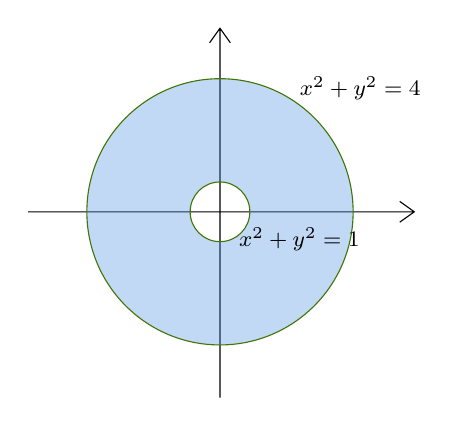
\begin{tikzpicture}[x=0.75pt,y=0.75pt,yscale=-1,xscale=1]
        %uncomment if require: \path (0,300); %set diagram left start at 0, and has height of 300

        %Shape: Axis 2D [id:dp2853296481227898] 
        \draw  (422.33,148.48) -- (608.33,148.48)(514.71,60.03) -- (514.71,238.03) (601.33,143.48) -- (608.33,148.48) -- (601.33,153.48) (509.71,67.03) -- (514.71,60.03) -- (519.71,67.03)  ;
        %Shape: Donut [id:dp2986115185015372] 
        \draw  [color={rgb, 255:red, 65; green, 117; blue, 5 }  ,draw opacity=1 ][fill={rgb, 255:red, 74; green, 144; blue, 226 }  ,fill opacity=0.34 ,even odd rule] (500.34,148.48) .. controls (500.34,140.54) and (506.77,134.1) .. (514.71,134.1) .. controls (522.65,134.1) and (529.09,140.54) .. (529.09,148.48) .. controls (529.09,156.42) and (522.65,162.86) .. (514.71,162.86) .. controls (506.77,162.86) and (500.34,156.42) .. (500.34,148.48)(450.57,148.48) .. controls (450.57,113.05) and (479.29,84.34) .. (514.71,84.34) .. controls (550.14,84.34) and (578.86,113.05) .. (578.86,148.48) .. controls (578.86,183.9) and (550.14,212.62) .. (514.71,212.62) .. controls (479.29,212.62) and (450.57,183.9) .. (450.57,148.48) ;

        % Text Node
        \draw (552,82.4) node [anchor=north west][inner sep=0.75pt]  [font=\footnotesize]  {$x^{2} +y^{2} =4$};
        % Text Node
        \draw (522.67,155.07) node [anchor=north west][inner sep=0.75pt]  [font=\footnotesize]  {$x^{2} +y^{2} =1$};
        \end{tikzpicture}
    \end{center}

    $z=f(x,y)=(x^2+y^2)^{\frac{1}{2}},\ f_x=\dfrac{x}{\sqrt{x^2+y^2}},\ f_y=\dfrac{y}{\sqrt{x^2+y^2}}$,

    hence $ds=\sqrt{1+(f_x)^2+(f_y)^2}dA=\sqrt{2} dA$,
    \begin{align*}
        \iint_S \rho(x,y,z) dS &= \iint_R \left(10-\sqrt{x^2+y^2}\right)\sqrt{1+(f_x)^2+(f_y)^2}dA\\
         &= \sqrt{2} \iint_R (10-\sqrt{x^2+y^2}) dA\\
         &= \sqrt{2} \int_0^{2\pi} \int_1^4 (10-r)\ r dr d\theta = 108\sqrt{2} \pi
    \end{align*}

    \newpage
    \subsection{Surface Integrals of vector fields: flux}

    

\end{spacing}
\end{document}
